\documentclass[11pt]{article}
\usepackage[english]{babel}
\usepackage[utf8]{inputenc}
\usepackage{fancyhdr}
\usepackage{graphicx}

\def\Name{Ran Liao}
\def\Topic{Statechart}

\title{\textbf{\Topic}}
\author{\Name}
\markboth{Notes on \Topic\ }{Notes on \Topic\ }
\date{\today}
 
\pagestyle{fancy}
\fancyhf{}
\rhead{\date{\today} }
\lhead{Notes on \Topic\ }
\rfoot{\thepage}

\textheight=9in
%\textwidth=6.5in
\topmargin=-.75in
%\oddsidemargin=0in
%\evensidemargin=0in
 
\begin{document}
\maketitle
\noindent\makebox[\linewidth]{\rule[8pt]{5in}{0.5pt}}

\section*{Overview}

A statechart shows states (specific values of attributes of objects), events that cause transitions between states (subject to guards), and actions taken by objects.

\section*{Example}

\begin{figure}[h]
	\centering
	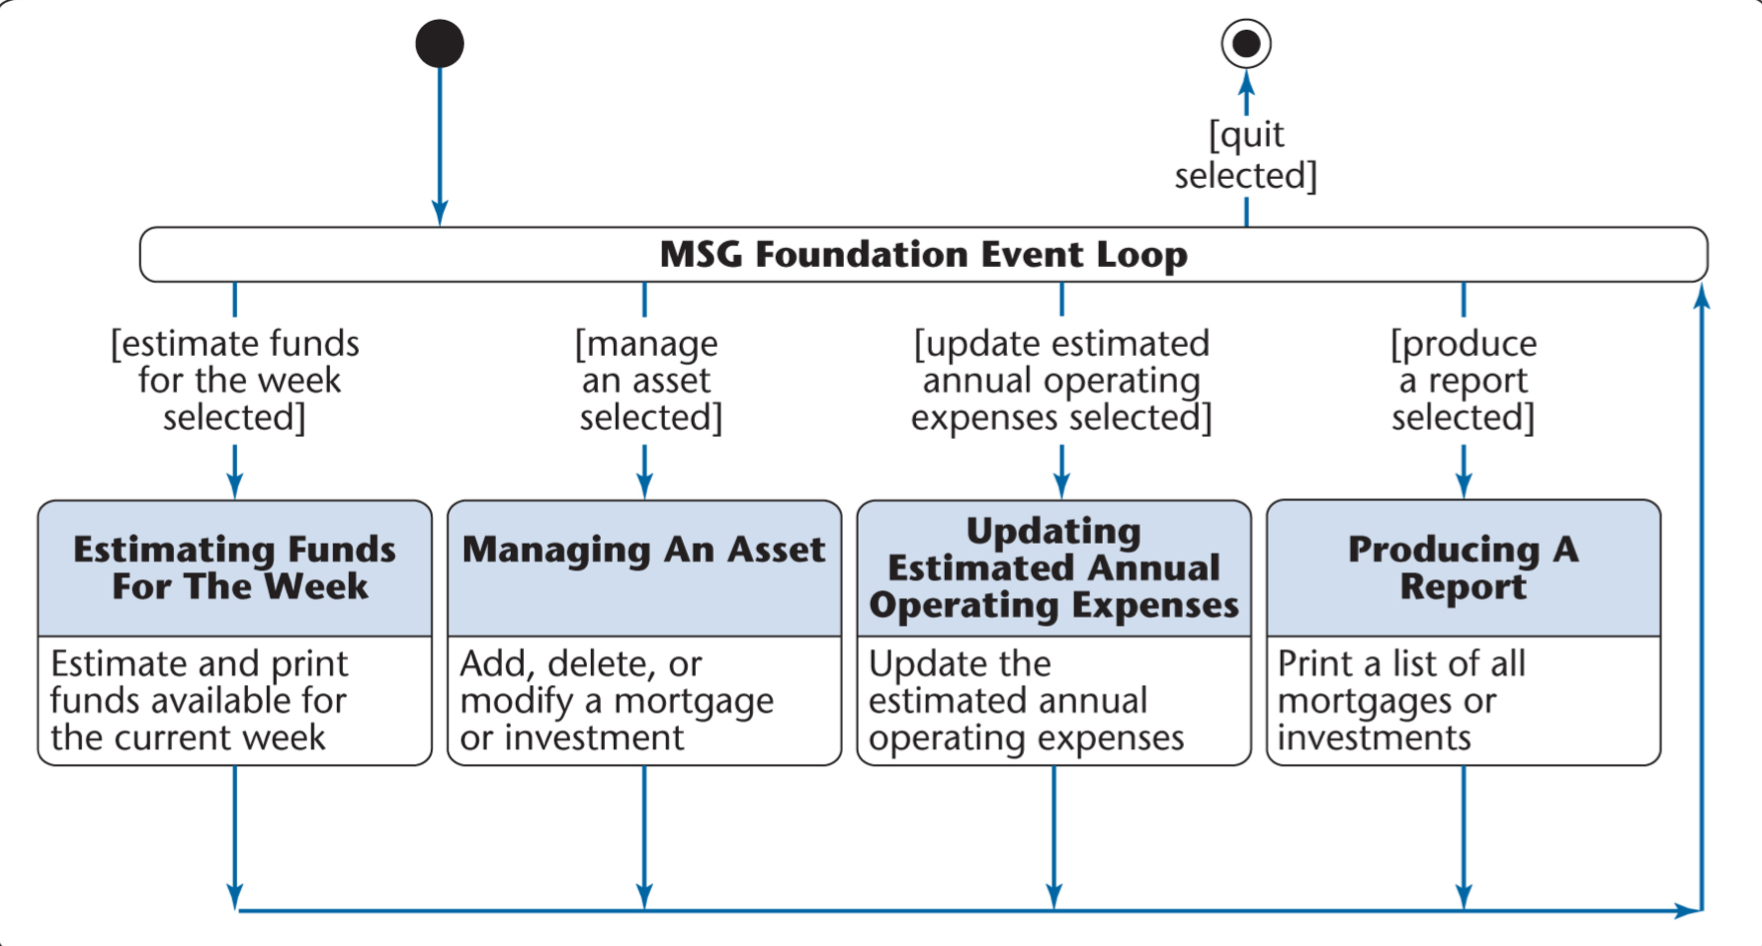
\includegraphics[width=0.9\linewidth]{images/Statechart.png}
	\caption{Statechart}
	\label{fig:Statechart}
\end{figure}


\end{document}